\documentclass{beamer}

\title{Example presentation}
\subtitle{Use theme and colortheme}
\author{Andrew Johnson}
\institute[Georgia Tech]{Georgia Institute of Technology}
\date{11 Nov, 2019}

\usepackage{tikz}
\usetikzlibrary{arrows}

\usetheme{atlanta}
\usecolortheme{yellowjacket}

\begin{document}

\frame{\titlepage}

\begin{frame}{Outline}
    \tableofcontents
\end{frame}

\section{Lists}

\frame{\sectionpage}

\subsection{Simple lists}

\begin{frame}{Lists}
    \begin{enumerate}
        \item{This is a numbered list}
        \item{Go up to three levels at most}
            \begin{enumerate}
                \item{Two is probably the best}
                    \begin{enumerate}
                        \item{But three works}
                    \end{enumerate}
            \end{enumerate}
    \end{enumerate}
    \begin{itemize}
        \item{Bulleted list}
            \begin{itemize}
                \item{Up to three tiers as well}
                    \begin{itemize}
                        \item{Leverage citations \cite{burdell_1999}}
                    \end{itemize}
            \end{itemize}
    \end{itemize}
\end{frame}

\section{Blocks and floats}

\subsection{Blocks}

\begin{frame}{Blocks}
    \begin{block}{Blocked}
        Good for highlighting important information
        \begin{itemize}
            \item{Can embed lists}
        \end{itemize}
    \end{block}
\end{frame}

\subsection{Tables}

\begin{frame}{Tables}
    \begin{table}
        \caption{Look at this table}
        \begin{tabular}{|l|r|}
            \hline
            Item & Value \\
            \hline
            Wigets & 100 \\
            Dodads & 12.3 \\
            \hline
        \end{tabular}
    \end{table}
\end{frame}

\subsection{Figures}
\begin{frame}{Figure}
    \begin{figure}
        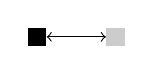
\begin{tikzpicture}
            \node[fill=black] (start) {};
            \node[fill=black!20] (end) [right of=start] {} edge[<->] (start);
        \end{tikzpicture}
        \caption{Kind of lame figure though...}
    \end{figure}
\end{frame}

\begin{frame}{References}
    \bibliography{reference.bib}
    \bibliographystyle{IEEEtran}
\end{frame}

\end{document}

